\documentclass[11pt,a4paper]{scrbook}
\usepackage{geometry}	
%\usepackage[backend=bibtex,style=numeric]{biblatex}
%\usepackage{ngerman}
%\usepackage[T1]{fontenc}
\usepackage[utf8]{inputenc}
\usepackage[style=numeric]{biblatex}
\bibliography{../PaperBib2}
\usepackage{colortbl}	
\usepackage{xcolor}
%\usepackage{soul}
\usepackage{amsmath}
\usepackage{graphicx}
\usepackage[outdir=../Graphen/]{epstopdf}
\usepackage{textcomp}
%\usepackage{floatrow}
\renewcommand{\figurename}{Fig.}
\usepackage[skip=0pt]{caption}
\captionsetup{format=hang}
\setcapindent{0pt}
\usepackage{subcaption}
\usepackage{scrhack}
%\renewcommand{\familydefault}{\sfdefault}
\definecolor{uhhred}{cmyk}{0,100,100,0}
\usepackage{tabularx}

\newcolumntype{L}[1]{>{\raggedright\arraybackslash}m{#1}}
\newcolumntype{C}[1]{>{\centering\arraybackslash}m{#1}}
\newcolumntype{R}[1]{>{\raggedleft\arraybackslash}m{#1}}

\usepackage{hyperref}
\hypersetup{linktocpage}

\begin{document}

\frontmatter
\newgeometry{centering,left=2cm,right=2cm,top=2cm,bottom=2cm}
\begin{titlepage}
\includegraphics[scale=0.3]{../Graphen/UHH-Logo_2010_Farbe_CMYK.pdf}
\vspace*{2cm}
\Large
\begin{center} 
      {\color{uhhred}\textbf{\so{BACHELORTHESIS}}}
%oder {\color{uhhred}\textbf{\so{MASTERTHESIS}}}
\vspace*{2.0cm}\\
{\LARGE \textbf{Improving the modelling of tempo and phoneme duration}}
\vspace*{2.0cm}\\
vorgelegt von
\vspace*{0.4cm}\\
Alexandra Krah
\end{center}
\vspace*{3.9cm}

\noindent 
MIN-Fakultät \vspace*{0.4cm} \\ 
Fachbereich Informatik \vspace*{0.4cm} \\ 
%Ggf. Professur/Institut \vspace*{0.4cm} \\
Studiengang: Informatik \vspace*{0.4cm} \\ 
Matrikelnummer: 6415559 \vspace*{0.8cm} \\ 
Erstgutachter: Dr. Timo Baumann \vspace*{0.4cm} \\ 
Zweitgutachter: Prof. Dr. Wolfgang Menzel

\end{titlepage}

\restoregeometry

\tableofcontents\thispagestyle{empty}

\mainmatter

\chapter{Introduction}
Some people speak faster, others speak slower, and all people speak sometimes faster and sometimes slower than they usually do. The tempo at which one speaks is what we call ``speech rate``. The fact that we understand people at all natural speech rates is certainly largely due to the quality features of sounds (phonemes) in the given language. However, if we have a perfect audio recording of speech, and play it faster or slower, we immediately notice how naturalness deteriorates. Synthetic speech shows a similar behavior when changing tempo. In both cases phoneme quality doesn't need to change. It is its duration that changes, along with some other suprasegmental features like pitch, and phrasal accents that do the trick. 

Attempts to improve the quality of speech synthesis when tempo changes also include linguistic processing, and phoneme length manipulation before the actual synthesis takes place. As mentioned in a patent documentation of Fujitsu Limited, phoneme length manipulation plays an important role in this context and one cannot rely on a linear adjustment function \cite{nishiike2008}. 

\subsection*{Scope}
Phoneme length adjustment is the aspect we wish to adress in this work. In particular, we want to find an algorithm for adjusting phoneme durations to the variation of the speech rate. The resulting phoneme duration should be close to the actual duration that occurs when speaking rate alters. This would be the same as playing an audio recording faster or slower. 

There are several models for phoneme duration approximation that work pretty well for some languages, German inclusive. However, they consistently don't take the speech rate into consideration, their performance level being acquired rather at a specific speech rate. When this varies, model performance deteriorates, like van Santen states for his model \cite{Santen1994}. Moreover, all of these models have an upper asymptote for their accuracy situated at less than 100\%. It has been suggested, that the influence of so-called ``macroscopic`` or para-linguistic \cite{Santen1994} factors should be examined in order to move this asymptote further up. Such a factor is speech rate, and we took the challenge of integrating it into a speech model. 

The purpose is therefore not to create another duration approximation model for TTS-systems, but to improve the algorithm of phoneme duration prediction by considering speech tempo. We argue therefore, that speech tempo produces a non-linear alteration of the phoneme durations.

Table \ref{tab:Question} visualizes our challenge: we want to put all available, i.e. visible information from the table in relation so that we can replace the question marks with values that are close to the real ones. Consequently, the modified speech unit sounds more natural when tempo varies. 

\begin{table}[htbp]
\centering
\begin{tabular}{|L{2.5cm}||*{4}{C{.8cm}|}|*{4}{C{.8cm}|}}
	\hline
			& \multicolumn{4}{c||}{ \textit{genau}} & \multicolumn{4}{c|}{ \textit{genau}} \\
	\hline
Phonemes		& g & @ & n & aU & g & @ & n & aU \\
	\hline
Durations (sec) & 0.05 & 0.07 & 0.05 & 0.11 & ?  & ?  & ?  & ? \\
	\hline
Speech rate $dur/\#phon$ & \multicolumn{4}{c||}{0.07} & \multicolumn{4}{c|}{0.11} \\
	\hline
\end{tabular}
\vspace{5mm}
\caption{Our inputs: duration of each phoneme in German word ``genau`` at a speech rate of 0.07 sec. corresponding to a word duration of 0.28 sec, and a new speech rate, 0.11 sec, equivalent to a word duration of 0.42 sec, for which we have the challenge of finding appropriate phoneme durations.}
\label{tab:Question}
\end{table}

Hoequist and Kohler observed already back in 1986 that the change in speaking tempo does not produce a linear change of the acoustic segments of an utterance (i. e. phonemes) \cite{Hoequist1986}. Indeed, if one simply ``stretches`` all phonemes in the same manner to accommodate a new speech rate, the result is rather disappointing, as one can see in Fig. \ref{fig:linear_approx}.

Across the paper we use the German SAMPA notations when referring to phonemes.
\begin{figure}[htbp]
	\centering
	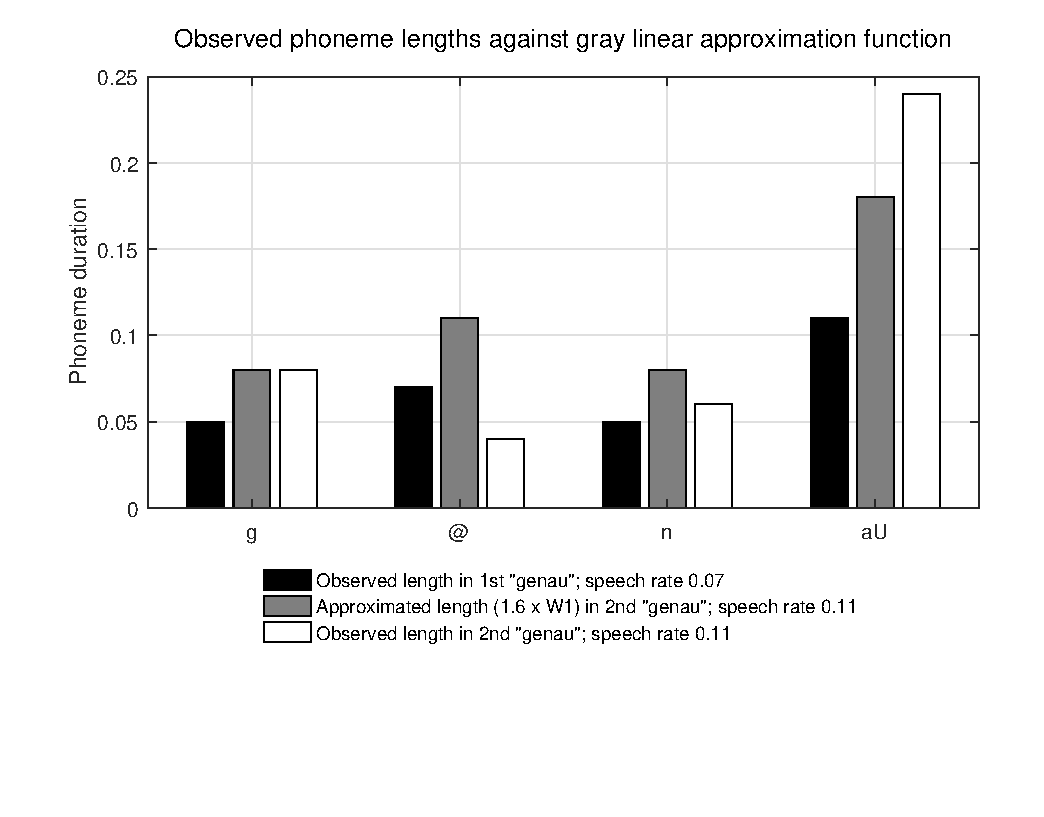
\includegraphics[trim=23mm 23mm 0mm 0mm, scale=0.7]{../Graphen/Linear_approx.eps}
	\vspace{4mm}
	\caption[Linear phoneme duration approximation]{This is a linear solution to the challenge presented in Table \ref{tab:Question}.}
	\label{fig:linear_approx}	
\end{figure}

\subsection*{Outline}
We start our challenge by defining our methods in Chapter \ref{chap_2}. In the following chapter we examine the available resources so that we can proceed with the actual task in Chapter \ref{chap_phonemes}, where we analyze the German phonemes. We dedicate Chapter \ref{chap_SR} to the challenge of finding an adequate speech rate definition for our database, and which can serve our purpose. Chapter \ref{chap_6:models} finally deals with phoneme duration prediction models and the challenge of finding a solution to our above presented issue.

\chapter{Means and Methods}
\label{chap_2}

\section{Machine Learning}
Machine Learning means building a program or model which can make predictions about an unseen dataset, like filling in missing information, based on data mining results from a given dataset. It consists of a so-called training phase, in which the training data is being processed by the selected machine learning method and hypotheses or models are formed. These can then be used to make predictions about new data. The training data consists of a set of instances, each of them being described by a feature vector. The training phase is followed by an evaluation phase, in which predictions about unseen data are being made and compared to the actual values. 

Data Mining means in foreground looking for patterns in data with the help of computers. Patterns are helpful for humans to understand data. They reduce the amount of data, and of available features to the relevant ones. Computers help process within resonable time amounts of data that would need years of manual processing.

We used machine learning to solve a task involving both classification and numeric prediction, and selected from its repertoire two model tree methods: M5P and REPTree. We chose these trees because: trees are easy to interpret, they can perform both classification and numeric prediction tasks, we could easily generate them using Weka, and they are the closest to classification and regression (CART) trees, also used in the literature \cite{Brinckmann_2003} for phoneme duration prediction, so we have data to compare with.

\subsection{Decision trees}
\label{dec_trees}
Decision trees divide the attribute space into well defined clusters, identified by a class name or a numeric value. In the first case we are dealing with a classification tree, in the second one with a regression tree. If one needs to combine the two methods, he/she may use a classification and regression tree, called CART, or a model tree. The advantage of trees is that new instances are easily assigned to a class, or a numeric value, or a linear model which leads to a numeric value, and they are easy to unterstand.

The \textbf{M5P model tree} is a decision tree based on the M5 algorithm introduced by Quinlan (1992). It builds an ordinary classification tree out of the selected attributes, and retrieves a linear regression model in each leaf out of the attributes contained in that specific subtree. Branching is realised based on the reduction of variation within the resulting subset.

A \textbf{REPTree} is a decision and regression tree similar to M5P, but optimized for speed. This means it sorts values for numeric attributes only once. 

Both trees cope well with missing data. However, both need large training sets in order to perform well.

\section{Preparing the Data}
A very important and time consuming step in data mining is data preparation, which is the next step after data collection. At this stage, one needs to assess the quality of the data, expressed as noise ratio, and the strategies for dealing with it. If the data used has been originally collected for another purpose, then it needs to be assessed in terms of features it contains, actually needed features, and organization, resp. reorganization of data to serve new purpose. 

Considering machine learning, it is straightforward that one needs to split the available dataset at least into two parts: a (bigger) training dataset, used for training the model, meaning to discover patterns in data, and a (smaller) test dataset, used for testing the performance of the model resulting from the machine learning process. We used the well-established split of 90\% training data and 10\% test data.

We explain how we prepared our data in chapter 3, dedicated to our database.

\section{Performance Evaluation}
Models produced by machine learning may have different performance levels, which may be evaluated in several ways. As they assess different features of the models, and treat outliers differently, we didn't want to rely only on one of them. Furthermore, we wanted to be able to compare the results with results presented in the literature. After studying the common evaluation methods used for other phoneme prediction models, we chose the following three: 
\begin{enumerate}
	\item \textbf{RMSE} or \textbf{root mean squared error} measures the differences between the numeric values predicted by a model and those actually observed: 
$RMSE = \sqrt{\frac{\sum(predicted-actual)^2}{n}}$. It is a very popular method for evaluating errors of a model, but it is very sensible to outliers.
	\item \textbf{MAE} or \textbf{mean absolute error} is similar to RMSE, but penalises outliers less. It is computed using the average of the absolute errors: $MAE = \frac{\sum\left|predicted-actual\right|}{n}$
	\item The \textbf{Pearson correlation coefficient}, a popular measure for continuous data, is a number between -1 and 1 that quantifies the correlation between two variables, each having a separate value set. We can interpret this as how much the variable movement through its value set corresponds to the movement of the other variable in its own value set. Values close to 1 mean that greater values of the one variable imply greater values for the second variable, negative values mean the two variables move in opposite directions, while values close to 0 mean there is no correlation between the two variables. However, one must keep in mind that correlation does not imply causality, so the presence of correlation between two variables does not mean that one of them has any influence on the other one. If we compare red Ferrari cars to blue Renault cars, one may find a correlation between car color red and car speed. However, this does not imply that red cars are generally faster.
\end{enumerate}
Throughout this work we consistently mean the Pearson's correlation coefficient whenever we speak about correlation.

\section{Tools}
We used \textbf{Weka} 3.8 for building and training the model trees for phoneme duration prediction. It is an open source freeware using a Java VM, and contains a collection of tools for all machine learning tasks we needed, from data pre-processing over classification and regression till model evaluation and data visualization.

In order to extract the needed information from our database, and put it in a form ready to use with Weka, we used self-made code written in \textbf{Python} 3.6. This is an easy to learn programming language with many features dedicated to statistical analysis and even machine learning. Most of the figures in this paper were produced in python as well.

\chapter{Corpora}
\label{chap_3}
Language related databases are called corpora, and for our purpose we needed one containing segmented and annotated German speech as a set of text files, so-called ``textual data``. Our minimum requirement for such a corpus was that it contains speech segmented at phoneme level, allowing us to calculate the duration of each phoneme occurence. The unit in which this duration is expressed is not relevant. As phoneme duration may be influenced by several factors, and we did not intent to do any further processing of the audio files, we also needed that this textual database contains enough information to identify following attributes: 

\begin{itemize}
	\item phrase boundaries
	\item word boundaries
	\item syllable boundaries
	\item phoneme identification
	\item vowel stress
	\item pauses
\end{itemize}

There are three corpora which we had at our disposal: (1) The Kiel Corpus of Read (\textit{PhonDat} or \textit{KCoRS}) and of Spontaneous Speech (\textit{KCoSS}), (2) Verbmobil, and (3) spoken Wikipedia. The first one contains two equal sized corpora of > 4 hours each: KCoRS, which is a collection of read speech, and KCoSS, which is a collection of spontaneous speech, both being manually segmented, a good indicator for good segmentation quality. However, as Pfitzinger \cite{Pfitzinger2002} also showed in his reassessment of the PhonDat-II corpus, for nowadays research the Kiel Corpus is rather small. Spoken Wikipedia is a new project comprising of a much larger collection of read speech. Unfortunately, the phoneme-level segmentation was not ready on time to evaluate in our project, so we chose Verbmobil.

\section{Verbmobil}
The Verbmobil corpus is a database of spontaneous speech containing a collection of appointment making dialogs, fully transliterated and annotated. This was an important point in selecting this database for our purpose, as phoneme duration is influenced by many factors, and the Verbmobil textual database provides most of them. We used 286 recordings from the last verbmobil phase (VM-II) created by 131 speakers. The total VM-II corpus used amounts to 11783 conversational turns representing recorded speech time of 15.5 hours. The ``symbolic data`` corresponding to each turn (e.g. phonetic transcription, segmentation, labeling, etc.) is captured in so-called ``par files``, representing files in the ``BAS Partitur Format`` \cite{Burger2000}. Our dataset included 604355 automatically labeled phoneme instances.

Drawbacks of this database come mainly from the characteristics of spontaneous speech. Following natural rules, speech rate often varies significantly inside a speech turn. This means one starts his turn at a normal speech rate, then gets to a point where he/she hesitates and gets slower, like when weighting different transport means to get to the appointment they are to agree upon. This results in the challenge of finding an appropriate description for the speech rate to be used for the modeling of phoneme durations across the corpus. We handle this issue of speech rate separately in chapter 5. Another challenge resulting from the structure of this corpus as a collection of dialogs is speaker variation. The exact coordinates of phoneme durations vary across speakers, as one can see in Fig. \ref{fig:speaker_cmp}, for the case of the phoneme \texttt{/a:/}.

\begin{figure}[htbp]
	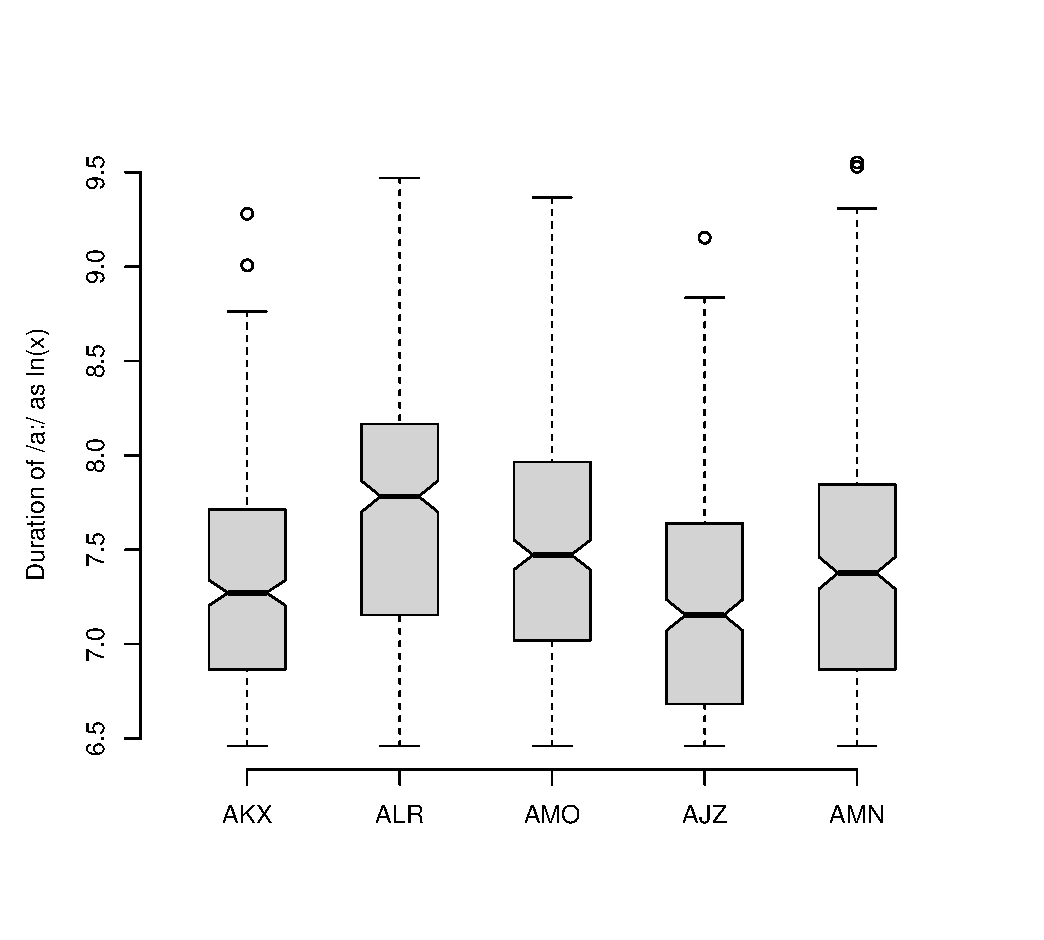
\includegraphics[width=0.6\textwidth]{../Graphen/Duration_of_a_5speakers.eps}
	\centering
	\caption[Phoneme length variation between speakers]{Overview of \texttt{/a:/} length on the 5 most frequent speakers. Phoneme length is expressed as the natural logarithm of the sample frequency. While the minimum duration is technically limited to an equal value corresponding to 0.04 sec, all other coordinates vary, e.g. maximum value has a variation of 0.14 sec between speakers AKX and ALR. The greatest median variation is 0.07 sec between speakers ALR (0.15 sec) and AJZ (0.08 sec).}
	\label{fig:speaker_cmp}
\end{figure}

\chapter{German phoneme system}
\label{chap_phonemes}
The phoneme inventory used in Verbmobil includes 52 classes defined according to the German SAMPA. However, only 49 of these occur in the examined corpus. The missing ones are \texttt{/2/} as in \textit{Ökonom}, and the nasals \texttt{/E$\sim$/} and \texttt{/O$\sim$/} as in the loanwords \textit{Teint, Saison}. Using the classical phonetic conventions, we can group these phonemes using a tree structure. The first branching splits them into vowels, consonants and a glottal stop, although the latter one is sometimes treated as a consonant \cite{Kohler1995}. Vowels represent 24\% of the total phoneme inventory analyzed. Further relevant groupings are discussed in subsections ``Vowels`` and ``Consonants``.

Pauses may be caused by and/or be quantitatively modified both by linguistic (e.g. phonological) and non-linguistic factors, like technical, psychological, and dialog dynamics. Consequently pause length variation needs to be treated separately from phoneme duration variation, as a not negligible large set of other factors are to be considered for this, such as dialogue dynamics, hesitations, or technical issues of the recording which all extend beyond the purpose of this work.

\section{Vowels}
Vowels are an important class with respect to tempo modelling, because they show a high degree of elasticity in terms of duration, and correlate well with the speech rate. The minimum value recorded for vowels lies at 0.03 sec, while their maximum is 2.3 sec. The variation inside the value group may be expressed in terms of standard deviation with a $\sigma$ value of 0.07 sec. However, most values lie within a much smaller range, and 75\% of the vowels are shorter than 0.1 sec. If we remove 1\% of the data at the higher end, $\sigma$ reduces to 0.05 sec and the maximum duration at 0.3 sec. After carefully analyzing some of the outliers, we decided to keep them. We observed that some vowels may last as long as one can hold breath, like in the case of \texttt{/a:/}. Due to this high elasticity, vowels are the best candidates to start working on any phoneme duration model, as they are extremely sensitive to duration influencing factors. 

One can say that vowels generally tend to get proportionally longer when the words themselves are spoken slower. We investigated this assumption by comparing the vowel duration inside words containing a specific number of phonemes, as well as the variation of the word time proportion occupied by them in such words. The results confirmed this hypothesis. We illustrate this in Figure \ref{fig:w_dur_vs_pho} on the word ``genau``, where you can see that the length of the diphthong \texttt{/aU/} changes proportionally to the word duration, while the other phonemes seem to be unaffected by word duration. This leads to the idea that at least some phonemes tend to occupy a specific steak (proportion) of the total word duration in words with a specific composition accounting for a linear correlation with word duration in such cases. Figure \ref{fig:boxplot_prop} shows the proportion distribution of diphthongs, the longest long vowel \texttt{/a:/}, its short counterpart \texttt{/a/}, and a plosive consonant \texttt{/b/} in words containing a total of three phonemes. As expected, the diphthongs occupy the greater steak, while the consonant the smaller one. This also means that it is a good idea to look for the correlation between vowels and speech rate. We obtained an overall correlation coefficient of $r = 0.72$ for vowels against speech rate. Inside the vowel group, we could identify the primary stressed vowels as the actual correlation owners, with a group correlation value of $r = 0.75$, while the unstressed and secondary stressed ones showed rather modest correlation values of $r = 0.56$, respectively $r = 0.47$. 

\begin{figure}[htbp]
	\noindent\makebox[\textwidth]{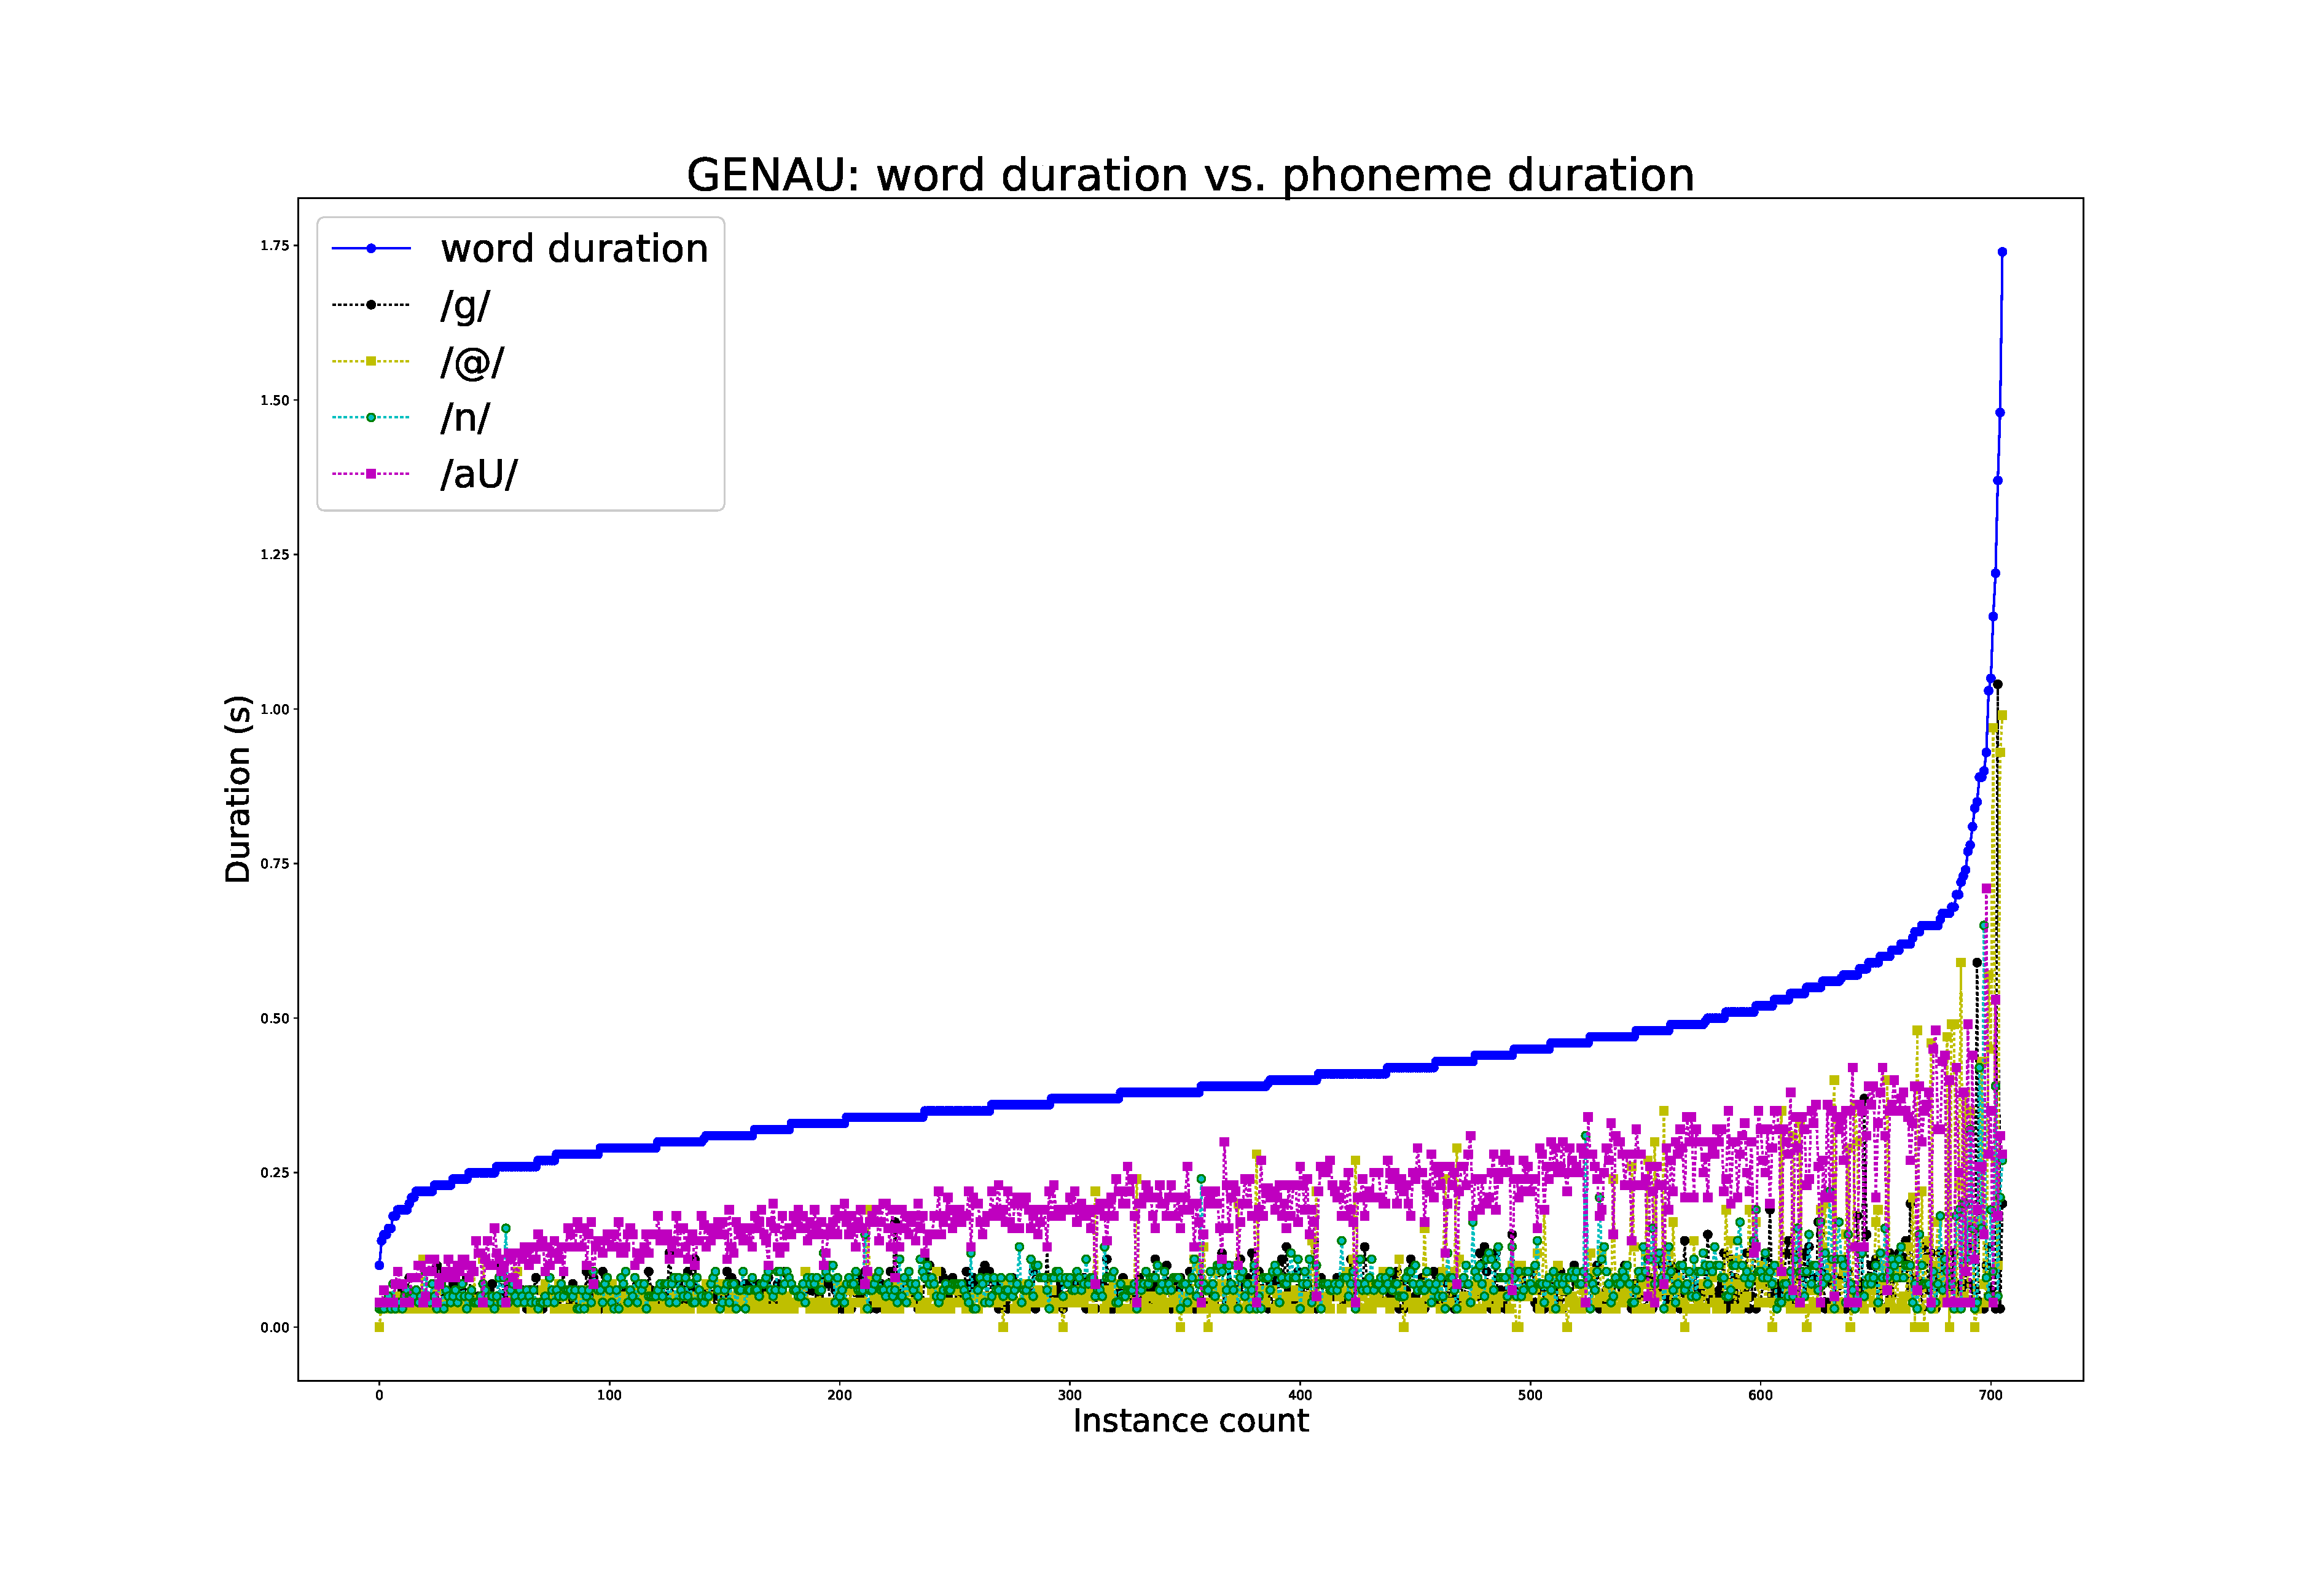
\includegraphics[trim=30mm 30mm 30mm 10mm, clip, width=\textwidth]{../Graphen/Stats_for_genau.eps}}
	\centering
	%\vspace{mm}
	\caption[Word duration of ``genau`` vs. its phoneme durations]{We ordered ascendingly the 706 occurences of the word ``genau`` based on word duration and ploted recorded durations of the component phonemes against it. The picture suggests clearly that the diphthong \texttt{/aU/} occupies a rather fixed steak of the total word duration, while the other phonemes show no adjustment to the increasing word total duration. }
	\label{fig:w_dur_vs_pho}
\end{figure}

We identified following vowel categories as being relevant for our purpose:

\begin{itemize}
	\item Diphthongs represent a slide between two vowels that are articulated together in a syllable. They are generally characterized by longer durations. German knows three diphthongs: \texttt{/aI/, /aU/} and \texttt{/OY/} as in \textit{Haus} \texttt{/haUs/},  \textit{heiß} \texttt{/haIs/} and \textit{moin} \texttt{/mOYn/}. We considered them as a separate group, as they are generally longer than all other phonemes.
	\item Schwa: most frequent vowel in German as well as in English. It is also called a reduction vowel \cite{Kohler1995}, as most of the other monophthongs tend to be articulated as schwa in non-stressed vowels. Verbmobil differentiates two types of schwa for the German language: \texttt{/@/} like in the last syllable of \textit{lesen} and \texttt{/6/} like in \textit{Leser}, where the reduced vowel is followed by an \texttt{/r/} in writing.
	\item Long vowels. As long vowels usually carry the primary stress, as some german phonetics manuals such as the one of Kohler \cite{Kohler1995} suggest, we considered the long vowels as a standalone subclass of vowels. The correlation value for the long vowel group is even greather than that of the primary stressed one, amounting to $r = 0.79$.
	\item Short vowels, in opposition to the above mentioned vowel categories, group phonemes that are to be considered as vowels from the point of view of their production, but which show a relatively low elasticity with respect to duration, if we compare them to the other three vowel groups.
\end{itemize}

\begin{figure}[htbp]
	\includegraphics[trim=15mm 0mm 15mm 0mm, width=.55\linewidth]{../Graphen/box3_oyauaiaab.eps}
	\centering
	\caption[Proportions of diphthong in 3-phoneme-words]{The time slice occupied by vowels in words of specific length  vary relatively little, indicating a possible linear correlation between their duration and the variation of word duration. Here you can see the difference in steak occupied by diphthongs next to the longest monophthongs \texttt{/a:/}, \texttt{/a/}, and a consonant \texttt{/b/}. The y-axis measures time in seconds.}
	\label{fig:boxplot_prop}
\end{figure}

Table \ref{tab:vowel_stats} below presents the main duration information regarding the above mentioned vowel classes that consolidates the discussion presented above.
\begin{table}[htbp]
\centering
%\vspace{10mm}
\begin{tabular}{|l|c|c|c|c|c|c|c|}

\hline
	 & Min value & Max value & Mean & St. Dev. & Q25 & Q75 & Count\\
\hline
\hline
Diphthongs  	& .04  & .71 & .12 & .06 & .08 & .15 & 8495\\
	\hline
Long vowels   & .04 & 2.3 &  .11 & .08 & .06 & .13 & 30425\\
	\hline
Schwa  &  .03 & 1.02 & .08 & .07 & .04 & .09 & 21637 \\
	\hline
Short vowels & .03 & .81 & .07 & .04 & .04 & .08 & 42570 \\
	\hline
\end{tabular}
\vspace{5mm}
\caption{Numeric information on the duration of the main vowel classes. The unit of the values presented in all columns except ``Count`` is second.} 
\label{tab:vowel_stats}
\end{table}

The vowel tree can be continued further down, introducing several further quality related features from the domain of the articulation manner, which leads to single phonemes at the leaves. It is good to have an overview on the articulation of vowels, i.e. on locating vowels according to their place of creation, and Fig. \ref{fig:vow_square} illustrates this very well. However, our purpose was to group vowels in order to get an overview about the phoneme durations for the beginning, so we don't go further down the tree. 

\begin{figure}[htbp]
	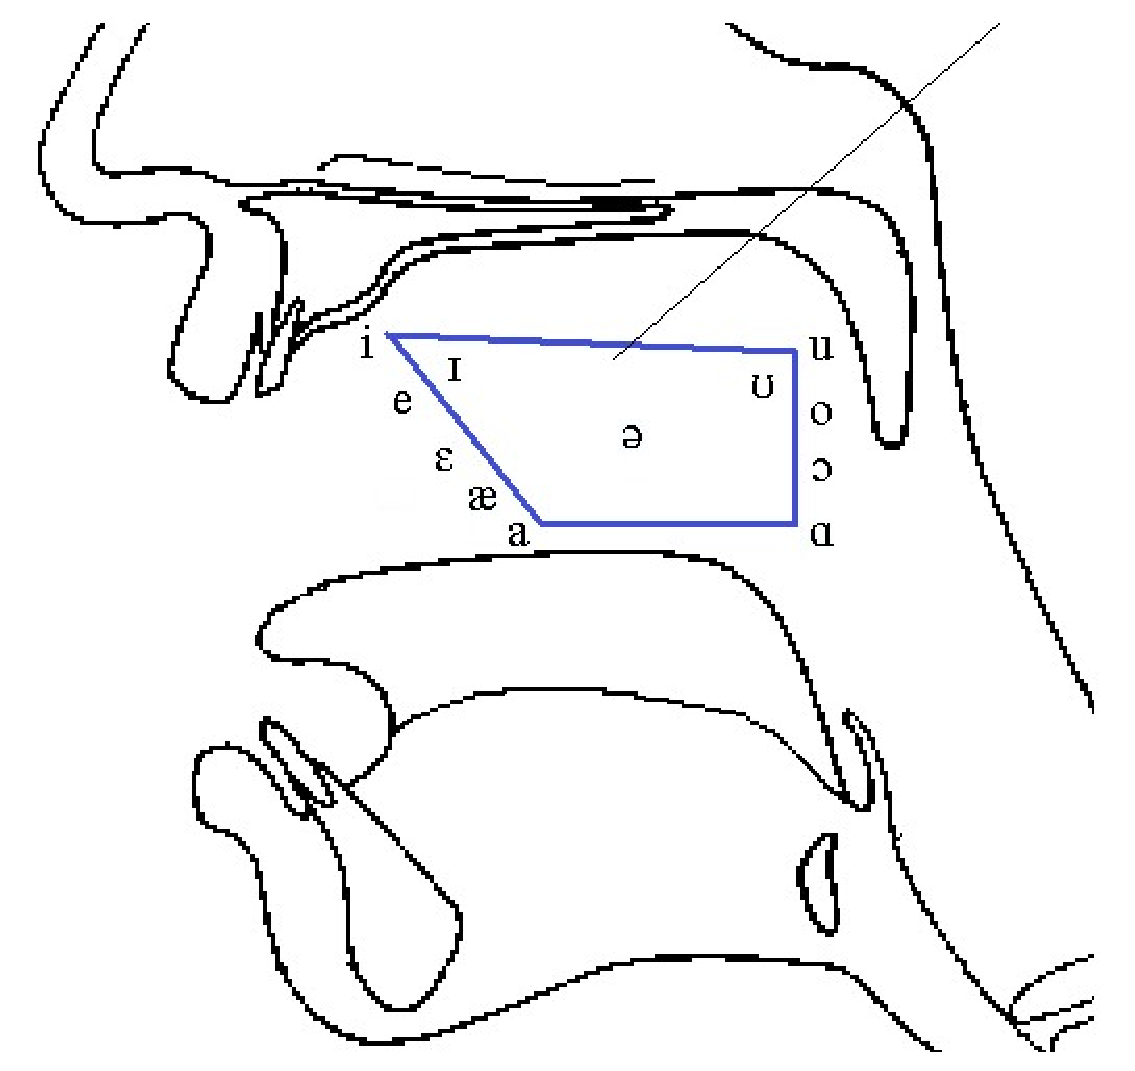
\includegraphics[width=.5\linewidth]{../Graphen/vow_art.eps}
	\centering
\vspace{5mm}
	\caption[Vowel square]{Vowels are produced by the air flow in an open vowel tract, and they differ based on the modification we add to the shape of this cavity. The only way for humans to produce such modifications are by moving the tongue and/or the lips. These changes are usually represented in the so-called vowel square, which may be further simplified to a vowel triangle. Here you can see how to place a vowel square containing the main vowels in the mouth cavity and how alone schwa lies in the middle of this square - for the production of schwa we don't need to act on the air flow. }
	\label{fig:vow_square}
\end{figure}

\section{Glottal stop}
\label{Q}
The glottal stop occurs 13 348 times and only word initially in our database, marked with \texttt{/Q/}. We decided to treat it separately because of its particular usage in German: it may occur only at the beginning of a word or a word stem and in front of a vowel. Some phonetic manuals don't event consider it a phoneme \cite{Ternes2012}. Furthermore, its acoustical properties make it look like a (filled) pause in speech, which represents a challenge for the transcription. As our files were segmented automatically, there is place for doubt about the accuracy of the collected data for \texttt{/Q/}.

However, unlike pauses we did consider it  for analysis, as it has an important communicative function as delimiter for words and morphemes. It is in fact one of the important clues which help hearer understand speech \cite{Ternes2012}. 

The information collected from our database show a very large variation of its duration from 0.04 sec. to 2.05 sec., with $\sigma = 0.06$, consistent with the official data on the complete VM-II. However, if we remove the upper 0.8 \% of the duration data, we obtain a dataset having only half of the mentioned variation with $\sigma = 0.03$ and a maximum duration of 0.3 seconds. We checked manually some of the largest outliers and they proved to be a result of wrong segmentation. Their real duration was within the first 2 thirds of the data.

\section{Consonants}
\label{cons}
In general, we can say that consonants present different degrees of elasticity, which are, however, generally lower than the ones of vowels.

Based on the correlation between phoneme duration and speech rate we created a subgroup of consonants containing the nasals and \texttt{/x/, /C/, /h/} with a relatively good correlation value $\geq 0.7$, and considered plosives to be an independent subgroup because of their consistently low correlation $\leq 0.42$.

A big surprize in the Verbmobil dataset was the huge duration variation of the plosive /t/, which was even greater than most of the fricatives. Evaluation of some samples showed this to be a result of wrong segmentation in the context /ts/, giving /t/ the longer duration and /s/ the shorter one. Another explanation would be that the phase before the release phase may indeed be relatively long.

Same as vowels, the consonant branch of the tree may be split further down into smaller categories. We chose to include them in our phoneme overview, as some of these categories proved to be relevant for the modelling of phoneme durations as well. Consequently, level 2 split of the consonant node shows following categories:
\begin{itemize}
	\item Plosives, which are generally short, due to their articulation characteristics. Their production involves two separate phases: closure, when the vocal tract is completely closed, and release, when the accumulated air flow is let out as in a burst. Considering this, it is straightforward, that the first phase may be longer, limited only by the human physiology, while the second one is technically extremely short. Some speech corpora, like PhonDat, label the two phases differently. Verbmobil doesn't, so we had to take them as a whole. We keep these considerations in mind, when referring to the special case of \texttt{/t/} that we found in our corpus.
	\item Fricatives, which show a duration variation almost comparable to that of vowels. This fact can also be explained by their production process: the vocal tract is not completely closed, but the air flow is forced out through a narrowing at some point in the vocal tract, so that a friction sound is produced.
	\item Nasals also show an elasticity comparable to that of vowels. Again this is explainable through their production: the oral passage is blocked, while lowering the velum, so that the air can escape through the nose. Nasals may also constitute the nucleus of a syllable, when the vowel gets reduced. German has three nasal consonants: /m/, /n/, /N/.
	\item Liquids, also called approximants, are produced by partial closure of the mouth produced by the thongue. German knows two liquids \texttt{/l/, /r/}.   One relevant feature is that they have the greatest freedom to occur in consonant clusters, that is a group of consonants belonging to the same syllable part. This also means that they must be particularly short, as we identified vowels to be the greater steak holders in word duration. Another fact we considered, is that \texttt{/r/} is relatively seldom in German, being often reduced to a schwa, and when it is articulated, then it is generally extremely short, which durations comparable to the ones of the glottal stop.
\end{itemize}

Plosives and fricatives may be split further down into voiced, if the vocal cords are participating in the production of the sound, and voiceless, when the vocal cords do not participate. We didn't analyse these groups in particular, as we focused on vowels. 

Table \ref{tab:cons_stats} below presents the main duration information regarding the above mentioned classes, sustaining our comments on them.
\begin{table}[htbp]
\centering
%\vspace{10mm}
\begin{tabular}{|l|c|c|c|c|c|c|c|}

\hline
	 & Min value & Max value & Mean & St. Dev. & Q25 & Q75 & Count\\
\hline
\hline
Plosives  	& .03  & 1.50 & .06 & .05 & .03 & .07 & 45477\\
	\hline
Fricatives   & .03 & 1.89 &  .06 & .05 & .03 & .08 & 51667\\
	\hline
Nasals  &  .03 & 1.46 & .08 & .08 & .04 & .09 & 39936 \\
	\hline
Liquids /l/ & .03 & 1.51 & .06 & .06 & .03 & .07 & 8019 \\
	\hline
Liquids /r/ & .03 & .46 & .05 & .03 &  .03 & .06 & 5453 \\
	\hline
\end{tabular}
\vspace{4mm}
\caption{} 
\label{tab:cons_stats}
\end{table}

\chapter{Speech rate}
\label{chap_SR}
Speech rate is a measurement of the tempo of speech, that is, how quickly someone speaks. This may be seen as a discrete (qualitative) measure, with discrete values such as \textit{slow}, \textit{normal}, and \textit{fast} or as a continuous one, with continuous numerical values. We opted for the continuous version, because it is quantifiable and so can be a useful input into a regression, see Section \ref{dec_trees} on decision trees.

Expressed mathematically, speech rate can be defined similarly to speed in spatial displacement, which would be distance covered by time. In the case of speech, distance is not counted in the spatial domain but in relevant linguistic units. Other than in the case of distance, the length of the speech units is not standardized, like kilometers, or miles, but have different lengths. Moreover its size is also expressed in units of time: phoneme \texttt{/a/} has the length of \textit{x} seconds, milliseconds, etc. This is why we chose to revert the speed calculating fraction, as you may see in Eq. \ref{eq:eq1}, and divide the total time by the number of units contained to obtain units of equal length. The measure of speech tempo is then given by the resulting size of the units. It is logical, that when someone speaks faster, the number of phonemes uttered in a given time interval is larger, and therefore their average length shorter. In the case of slow speech the opposite is true, so this is a good measure for speech tempo.

Next, we need to choose an adequate time interval to calculate speech rate for. As we are interested in comparing the phoneme duration at different speech rates, one global speech rate calculated on the entire corpus would be inappropriate. In addition, the fact that our corpus contains only spontaneous speech suggests there is speech tempo variability also inside speech turns, and even inside prosodic phrases, as you may see in Figure \ref{fig:SR_example}, so we decided to get very local and calculate speech rate at word level. 

\begin{figure}[htbp]
	\centering
	\noindent\makebox[\textwidth]{\includegraphics[trim= 53mm 0mm 70mm 70mm, clip, width=.83\paperwidth]{../Graphen/SR_example.eps}}
	\vspace{-25mm}
	\caption[Example of speech rate variation inside a turn]{Transcription of speech turn no. 22 of speaker AAJ in dialogue g001. The closer the points are to one another, the faster he speaks. Orange lines mark prosodic boundaries, delimiting prosodic phrases. You can see great variation in speech tempo across this speech turn, as well as inside single phrases.}
	\label{fig:SR_example}
\end{figure}

The units to be counted inside given time interval, which is in our case the duration of a word, may be phonemes, or syllables. In the literature \cite{Pfitzinger1998} we also found mentions about a relative speech rate, which combines speech rate calculated for two different units: phonemes, and syllables. As our corpus shows a very large amount of 1- and 2-syllable words, taking phonemes as unit seems to be the most reasonable option. Therefore, we used speech rate defined as: 

\begin{equation}
\label{eq:eq1}
	SR = \frac{word \quad duration}{phoneme\quad count}
\end{equation}

An additional measure we used to evaluate how well a speech rate calculating formula may suit our purpose was the correlation value between speech rate and phoneme duration. You may see a listing of the Pearson correlation values in Table \ref{tab:SR_corr} as well as a scatter plot of the best suiting result in Figure \ref{fig:wsr}. As long vowels proved to be the most sensible to the variation of the speaking tempo, we present below the values obtained for this group, together with the speech rate calculated at different segment sizes.

\begin{table}[htbp]
\centering
\vspace{10mm}
\begin{tabular}{|l|l|c|}
\hline
Segment	 & Formula & Correlation coefficient (Pearson)\\
\hline
\hline
Turn	& $turn\_dur/phon\_count$ & 0.73 \\

\hline
Phrase  & $phrase\_dur / phon\_count$ & 0.56\\
	\hline
Word  & $word\_dur / phon\_count$ &  0.80\\
	\hline
\end{tabular}
\vspace{4mm}
\caption {Duration of long vowels vs. speech rate calculated at turn, phrase, and word level} 
\label{tab:SR_corr}
\end{table}

\begin{figure}[htbp]
	\centering
	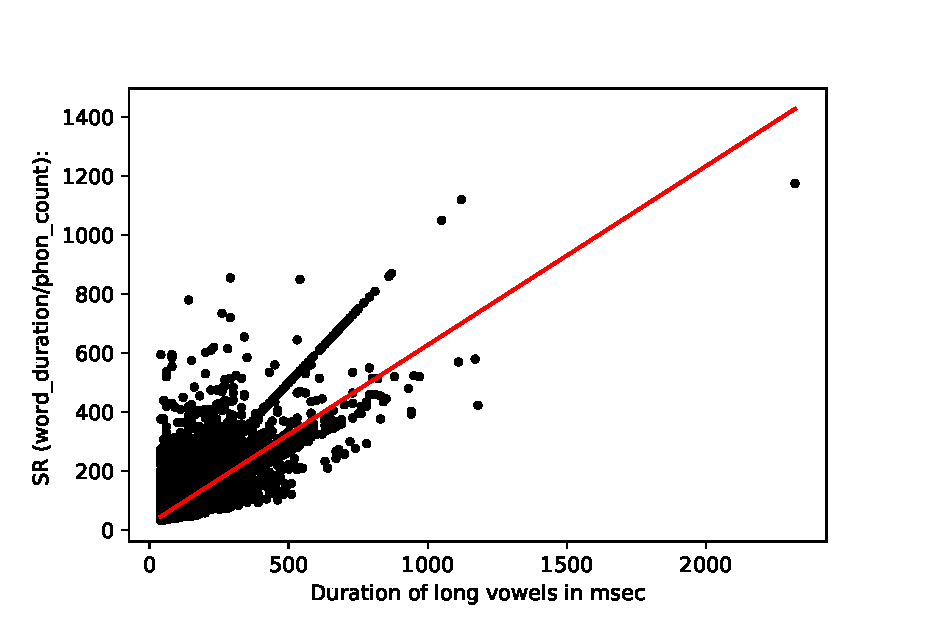
\includegraphics[width=.8\textwidth]{../Graphen/SR4.eps}
	\vspace{4mm}
	\caption[Speech rate vs long vowel duration]{Long vowel durations plotted against their respective speech rate (msec).}
	\label{fig:wsr}
\end{figure}

\chapter{Phoneme duration prediction models}
\label{chap_6:models}
There are several duration prediction methods in use: 
\begin{itemize}
	\item Klatt \cite{Klatt1979} is a rather simple method developped originally for American English. It multiplies a so-called inherent duration of given segment with a context dependent factor value and adds this to a segment specific minimal duration. Then the duration is estimated by adjusting the change coeficient successively for different factors, 11 of them being suggested by Klatt. These account for 84\% of observed total variance in segmental durations. The challenges of using this method reside in finding an appropriate inherent duration, adapting the Klatt factor values to the German language, and chosing the minimal duration to use.
	\item CART \cite{Riley1992} is a binary classification and regression tree with questions about the influencing factors at nodes and predicted values at the leaves. It allows consideration of both categorical and continuous factors, is quite simple and easy to interpret, in contrast to e.g. neural networks, and has a good time complexity of N*logN. The challenge of selecting an appropriate feature set is solved statistically. One drawback is that it needs a huge amount of training data in order to perform well. Also its performance deteriorates significantly with noisy or sparse training data \cite{Moebius1996}.
	\item Sums-of-products (SoP) proposed by van Santen \cite{Santen1994} generalizes the formula proposed by Klatt and uses a decision tree to group factors acting in the same direction, either lengthening or shortening the phonemes, so their effects add up (amplificatory interactions). In fact, the most important part and main challange of this model is to find an appropriate combination of factors to be used for specific phoneme groups. He didn't use speech rate as a factor, but observed that the performance of the model deteriorates when the speech rate changes. The advantage of this solution is that is copes well with noisy or missing data, and works well with much less training data than CART \cite{Moebius1996}. The application of this model for the German language by Möbius and van Santen using the PhontDat database resulted in an overall correlation coefficient of 0.896.
	\item Neural networks. Riedi \cite{Riedi1995} implemented a feed-forward neural network with two hidden layers for the prediction of phoneme durations and obtained a slightly better correlation coefficient than CART of 0.89 vs. 0.86. The drawback of this model is its intransparency.
\end{itemize}

Brinckmann and Trouvain \cite{Brinckmann_2003} compared Klatt and CART methods for predicting segment duration using the PhonDat database. Their results show a significantly better performance of CART over Klatt, with values of 0.86 vs. 0.79 for the correlation coefficient, consistent with previous results. However, they also report a strong influence of  the quality of the input data on the model performance.

\section{Method}
Our starting premise was that phoneme durations are being influenced by the speaking rate. In addition to this, we assumed that this influence is not equal on all phonemes, and on all situations, and therefore not linear. So we formulated our aim as to investigate the influence of speech rate on the duration of different phonemes and find a way of using this information to improve the performance of phoneme prediction models. 

In order to achieve this aim, we first examined the phonemes with respect to their duration. We found out that the classical phonetics book grouping of phonemes is not respected in terms of duration. There are consonants like \texttt{/N/}, and \texttt{/m/} which may be longer than some long vowels, and long vowels which are shorter than some short vowels or even several consonants, like \texttt{/y:/}. If one would apply a clustering method on phonemes to group them on seven classes based on their duration interval coordinates using, say k-means method, the resulting groups would certainly differ from those listed in Chapter \ref{chap_phonemes}.  

Therefore we decided to capture phoneme identity in our model as well, although it inflates the number of attributes and attribute values to compute. The relation between phoneme duration and factors other than speech rate was treated only marginally, as these have already been extensively examined in the literature on various corpora. For the German language, intuition aside, we have information on such factors provided by: Kohler \cite{Kohler1992}, Riedi \cite{Riedi1995}, Moebius \cite{Moebius1996}, and Brinckmann \& Trouvain \cite{Brinckmann_2003}, who applied some of the existent segment duration models to the German language. At this stage, we considered such factors only to the extent they might have helped identify groups of phonemes that may be best suited to evaluate the influence of speech rate. Such a factor is primary stress, which creates a group of very elastic vowels, which are therefore also sensitive to changes in speech tempo.

Then we looked for a definition of speech rate that can be used to model phoneme durations. This supposed the presence of a good correlation between speech rate and phoneme duration, at least for some phoneme groups. We explained our choice whith respect to this in Chapter \ref{chap_SR}. 
The fact, that speech rate doesn't show any correlation with some phonemes, like \texttt{/r/}, while it has a pretty good correlation with others, like \texttt{/a:/} suggests the need for classification in whichever model we choose.

\section{Experiment}
In order to test whether adding speech rate information really improves the predictions of a phoneme duration model, we tested the same model with and without the speech rate feature. We chose a tree model, because it is simple to implement, and to interpret. One can easily examine this kind of model to see which features are being used, and which weights they bear. 

For the sake of comparison, and to see whether we lie on the right track, we created at the beginning two basic models: 

\begin{enumerate}
	\item The first one predicted the phoneme duration as the mean of its durations across the whole corpus. 
	\item The second one built a two level tree, which split the root on the 49 realized phonemes, and then each phoneme on two specific speech rate values. The leaves contained three predicted values for each phoneme. These values were calculated using the mean duration of the specific phoneme across the corpus modified or not by a proportion of its standard deviation, based on the speech rate value split. 
\end{enumerate}

As the results of the initial two models were encouraging, we proceeded with a ``real`` model. For this, we reconstructed to a great extent a previous experiment \cite{Brinckmann_2003} that used a CART tree to predict phoneme duration, and reached good approximation values. By using this model we also had the advantage of having a reference for comparison. There is only one feature out of the 19 used in that experiment, which we could not recreate: degree of word accentuation. We lacked prosodic information for doing this. However, we tried to capture this kind of information by adding two extra word type classes: emphatic function words, like interjections and answer particles, and emphatic content words, like proper names and spelled items. For such words it is generally known that they usually carry phrasal stress.

Next, we pruned the used feature space by using two feature selection algorithms: forward and backward feature selection. Their principle is easy to understand and they are available in Weka. After pruning, the \textit{word} related features got completely eliminated, together with \textit{syllable-place-in-word} and \textit{articulation-of-realised-previous phoneme}. Consequently, following features were selected:

\begin{itemize}
	\item PHONEME INSTRINSIC FEATURES

	\begin{itemize}
		\item phoneme id: all 52 phoneme definitions used in Verbmobil
		\item phoneme type: vowel, or consonant
		\item articulation manner: vowel, plosive, fricative, nasal, lateral, approximant, other
	\end{itemize}

	\item SYLLABLE RELATED FEATURES

	\begin{itemize}
		\item position of phoneme in syllable: initial, final
		\item syllable part containing current phoneme: onset, nucleus, coda, single-phoneme-syllable
		\item lexical stress of the syllable (using the stress type of the nucleus vowel)
	\end{itemize}

	\item PHONEMIC CONTEXT

	\begin{itemize}
		\item previous phoneme type: vowel, consonant, or none
		\item following phoneme type: vowel, or consonant, or none
		\item articulation manner of following phoneme: vowel, plosive, fricative, nasal, lateral, approximant, other, none
		\item if following phoneme is voiced: yes, no, or none
		\item syllable part to which following phoneme belongs: onset, nucleus, coda, single-phoneme-syllable
	\end{itemize}
\end{itemize}

Note that all features refer to actually realised units in speech. We also had to reduce the amount of data used for the model to 58\% of the total corpus, due to capacity limitations imposed by Weka on our system. 

To this collection of features we added \textit{speech rate} in the second phase and compared the results. 

\section{Results}
\label{chap_6:results}
We trained and evaluated both a M5P and a REPTree model. The results were very similar, so we list here only the results obtained using the model tree M5P, as they were slightly better. As can be seen in Table \ref{tab:perfM}, adding the speech rate feature caused a significant improvement on all our models. 

\begin{table}[htbp]
\centering
%\vspace{10mm}
\begin{tabular}{|l|c|c|c|c|c|}

\hline
	 & Basic - SR & Basic + SR & M5P - SR & M5P + SR & CART\\
\hline
\hline
Correlation coef 		& .42  &  & .50 & .79 & .86 / .83\\
	\hline
MAE  &  31.02 & & 34.21 & 25.19 & 22.46 / 21.40\\
	\hline
RMSE  &  47.09 & & 62.91 & 44.70 & NA \\
	\hline
\end{tabular}
\vspace{4mm}
\caption{Overview of the performance results of 3 models with (+) and without (-) speech rate (SR). CART is the model created by Brinckmann \& Trouvain \cite{Brinckmann_2003}. The two values in the CART cells represent the performance obtained for 2 different speakers. RMSE was not reported for this model.} 
\label{tab:perfM}
\end{table}

However, the performance of our model tree is weaker than the performance of the CART model built by Brinckmann \& Trouvain \cite{Brinckmann_2003}. This is explainable if we consider the nature of the used datasets. The CART tree used PhonDat, a rather homogenous dataset in terms of speech rate and number of speakers. Furthermore, the model was trained and tested separately on data produced by one speaker. The reported results show even for PhonDat a difference in performance between speakers. Another aspect that can have a great impact on model performance is the quality of the input data. While PhonDat was manually segmented and annotated, Verbmobil was processed automatically using the MAUS segmentation system. When evaluating outliers we found many examples of wrong segmentation, as we also discussed in Sections \ref{Q} and \ref{cons}.

On the other hand, our model tree shows robustness with respect to factors like inter-speaker variability and speech rate. The results obtained for a test set containing data from a speaker not included in the training data were similar to those obtained on known speakers on terms of correlation coefficient, and showed less error rates, as can be seen in Table \ref{tab:perfM5P}. Moreover, if the model is to be evaluated on data produced by only one speaker, it produces good results even when using less than 10\% of the amount of data used to train on the multiple speaker corpus. The most frequent speaker in our database still only has 185 recorded turns, consisting of 9315 identifyiable uttered phonemes, which represent 0.02\% of the total phoneme instances in our corpus, so we could not test our model on a larger dataset of a single speaker. In comparison to this, the dataset used for CART contained 624 sentences, and a total of 4932 orthographically different words, which results in more than a double sized corpus.

\begin{table}[htbp]
\centering
%\vspace{10mm}
\begin{tabular}{|l|c|c|c|c|}

\hline
	 & \shortstack{Train: whole \\ Test: unseen speaker} & \shortstack{Train\&Test (+SR): \\ speaker AKX} & \shortstack{Train\&Test (-SR): \\ speaker AKX} \\ 
\hline
\hline
Correlation coef 		& .76   & .75 & .63 \\
	\hline
MAE  &  22.91 & 22.47 & 26.95 \\
	\hline
RMSE  &  40.36 & 33.87 & 40.30 \\
	\hline

\end{tabular}
\vspace{4mm}
\caption{Overview of the performance of our M5P model tree on different training and test sets.} 
\label{tab:perfM5P}
\end{table}

\chapter{Conclusion and Outlook}
Speech tempo is an important feature of natural speech, which produces lengthening or shortening of the speech units with reference to some ``standard`` speaking tempo. Our experiment shows that we can trace this influence at phoneme level, where it produces a non-linear modification in terms of duration of individual phonemes. Moreover, we have seen that adding a feature of tempo to a phoneme duration prediction model resulted in a significant improvement of model performance, even with a significant quantity of noise in the input data, as we stated in the discussion of our experiment results in Section \ref{chap_6:results}. 

The main difficulty we encountered was to find an appropriate definition of speech rate to be used in our models. Our definition considers the structure of the corpus used and the purpose it needs to serve. In addition, it did produce a significant improvement of the model used, so it may be used in phoneme duration prediction models. However, a universal definition of speech rate, applying to different corpora, would be desirable.

Future work would be to train and test such a model using the speech rate feature on data with a highly reduced amount of noise, which should result in an improved performance. 

A further possible improvement may achieved considering Koreman's observation \cite{Koreman_2006} on speech rate. He showed that perceived speech rate is influenced by the listener's knowledge of the expected articulations for a particular utterance, therefore it makes a difference if all expected phones are also articulated or not. Consequently, one could compare speech rate considering only articulated vowels/syllables, as well as considering both realized and intended phonemes, testing both methods with a given model. One possible result of such an approach would be the prediction of phonemes reaching $duration = 0$ at specific speech rates, which means predicting phoneme drop phenomena. In spontaneous speech, the word and syllable boundaries change, and this change influences other phonetic aspects such as stress, syllable duration, phoneme duration.

More generally, we spoke about improving the quality of rendered speech under varying tempo. Correct phoneme length prediction is just a step when improving the speech quality retrieved by audio programs when the rendering speed is modified, which we adressed in this work. However, when tempo changes in natural speech, other speech characteristics are being modified as well, like prosody, pitch, and phoneme quality, which cannot be simulated only by modifying the phoneme duration. Therefore, making speech sound natural while modifying the rendering speed needs to consider and adjust these other features too, implying further work to investigate changes of these factors produced by speech rate modification.



\printbibliography
\backmatter 

\thispagestyle{empty}

\vspace*{\fill}
\pagestyle{empty}
{\normalsize
\begin{center}\textbf{Eidesstattliche Erklärung}\end{center}
Hiermit versichere ich an Eides statt, dass ich die vorliegende Arbeit im Bachelorstudiengang Informatik selbstständig verfasst und keine anderen als die angegebenen Hilfsmittel – insbesondere keine im Quellenverzeichnis nicht benannten Internet-Quellen – benutzt habe. Alle Stellen, die wörtlich oder sinngemäß aus Veröffentlichungen entnommen wurden, sind als solche kenntlich gemacht. Ich versichere weiterhin, dass ich die Arbeit vorher nicht in einem anderen Prüfungsverfahren eingereicht habe und die eingereichte schriftliche Fassung der auf dem elektronischen Speichermedium entspricht.
\vspace*{1cm}\\
Hamburg, den 06.04.2017
\hspace*{\fill}\begin{tabular}{@{}l@{}}\hline
\makebox[5cm]{Vorname Nachname}
\end{tabular}
\vspace*{3cm}

}
\vspace*{\fill} 
\end{document}